\documentclass[12pt,a4paper]{report}
\usepackage{graphicx}
\usepackage{amsmath}
\usepackage{fancyhdr}
\usepackage{cite}
\usepackage{framed}
\usepackage{a4wide}
\usepackage{float}
\usepackage{epsfig}
\usepackage{longtable}
\usepackage{enumerate}
\usepackage{afterpage}
\usepackage{multirow}
\usepackage{ragged2e}
\usepackage{gensymb}
\usepackage{amsfonts} 
\usepackage[left=3.5cm,top=1.5cm,right=3cm,bottom=3cm]{geometry}
\usepackage{setspace}           
\usepackage{float}
\usepackage{txfonts}
\usepackage{lipsum}
\usepackage{tikz}
\usetikzlibrary{calc}
\usepackage{subfiles} % Best loaded last in the preamble


\newcommand{\Usefont}[1]{\fontfamily{#1}\selectfont}

\usepackage{lscape} % for landscape tables
\renewcommand{\baselinestretch}{1.7} 

\usepackage{blindtext}
\usepackage{xpatch}
\usepackage{url}
\usepackage{leqno}
\usepackage{subcaption}

\linespread{1.5}
\usepackage[intoc, english]{nomencl}
\hyphenpenalty=5000
\tolerance=1000
\usepackage[nottoc]{tocbibind}
\bibliographystyle{IEEEtran}
\renewcommand{\bibname}{References}

%********************************************************
%*********************Figures*****************************
% Save all figures in the folder figures and include them in your 
% report using the command \includegraphics{figure-name}

\graphicspath{{figures/}}

% figure files can be in jpeg,jpg, png or pdf formats
%*******************************************************************


\begin{document}
	
	
%****The entries in this section are to be filled in by the student with appropriate values *************

% These values are used thorough out the report 
% please fill in the appropriate values

\gdef \title{Sample Report Title} % Seminar title
\gdef \author{Abrar Ahmed chhipa}	 %student name
\gdef \rollno{22ETCEX001} %KTU Reg No
\gdef \acadyear{2021 - 21} % Academic year
\gdef \month{December 2021} %Month of Report submission
\gdef \date{21-12-2021} %Date of signing the declaration
\gdef \dept{Electrical Engineering} %Department
\gdef \deptabbr{Dept.of EE} %Dept name abbreviation
\gdef \degree{Bachelor of Technology} %degree
\gdef \branch{Electrical Engineering} %branch
\gdef \college{Techno India NJR Institute of Technology}
\gdef \collegeplace{Udaipur}

\gdef \guide{Dr. Abrar Ahmed Chhipa} %Project guide
\gdef \guidedes{Assistant Professor}%Project guide designation

\gdef \semcordinatorA{Mr. Rajkumar Soni}% Project coordinator 1 
\gdef \semcordinatorAdes{Assistant Professor}% Project coordinator 1 designation

\gdef \semcordinatorB{Prof. Seminar coordinator 2} % Project coordinator 2 
\gdef \semcordinatorBdes{Assistant Professor}% Project coordinator 2 designation

\gdef \hod{Dr. Prakash Bahrani} %Head of Department
\gdef \hoddes{Professor and Head} %HOD designation
%*******************************************************************
% The font pages. The source tex files are there in the folder
%==================================coverpage.tex================================


\newenvironment{coverpage}
\thispagestyle{empty}
\begin{titlepage}
\subfile{design_cover}
	\begin{center}
		{\Usefont{phv} \Large \bf \title \par}
		\vspace*{40pt}
		\large \em \Usefont{pzc}{ 
			A Major Project Report \par
			Submitted to the Rajasthan Technical University\\
			in partial fulfillment of requirements for the award of degree}\\ [.15\baselineskip] \par
		\Usefont{ppl} {\bfseries  \degree}\\
		in\\
		{\Usefont{ppl} {\bfseries \branch}}\\
		by\\
		\bf {\author}\\
		\bf{\rollno}
		\vspace*{40pt}
		\centering
		\begin{figure}[h!]
			\centerline{
\includegraphics[scale=0.8]{logo_college.jpg}}
		\end{figure}
		
		\vspace{\stretch{0.5}}
		\large{\bf DEPARTMENT OF ELECTRICAL ENGINEERING} \par
		\bf{TECHNO INDIA NJR INSTITUTE OF TECHNOLOGY} \par
		\bf{UDAIPUR, RAJASTHAN} \par
		\bf{\month}
	\end{center}
\end{titlepage}	
 %Unless essential Do not edit this tex file



%%********************Certificate*******************

% To print name of only the seminar coordinator 1 in the certificate page
%==================================certificate1.tex================================
% To print name of only the seminar coordinator 1 in the certificate page

\newenvironment{certificate1}

	\newpage
	\begin{center}	
		%\vspace{1.5cm}
		
		\textbf{DEPARTMENT OF ELECTRICAL ENGINEERING}\\	
		\textbf{TECHNO INDIA NJR INSTITUTE OF TECHNOLOGY}	
		\textbf{UDAIPUR, RAJASTHAN}
		
		\textbf{\acadyear} 
	\end{center}
	
	\begin{center}
		
\includegraphics[scale=0.8]{logo_college.jpg}	
	\end{center}
	\begin{center}
		\textbf{CERTIFICATE}
	\end{center}
	
	This is to certify that the report entitled \textbf{\title} submitted by \textbf{\author}\hspace*{2pt}(\rollno), to Department of \branch in partial fulfillment of the B.Tech.\ degree in \textbf{\branch}\hspace*{2pt} is a bonafide record of the seminar work carried out by him under our guidance and supervision. This report in any form has not been submitted to any other University or Institute for any purpose.
	
	
	\begin{singlespace}
		\vspace*{2cm}
		\begin{table}[h!]
			\centering
			\begin{tabular}{p{7cm} p{1.5cm} p{7cm}} 
				\textbf{\guide} && \textbf{\semcordinatorA} \\
				(Project Guide) &&  (Project Coordinator)\\
				\guidedes & & \semcordinatorAdes\\ 
				Dept.of EE && Dept.of EE\\ 
				Techno India NJR Institute & &Techno India NJR Institute\\
				of Technology &&of Technology\\
				Udaipur, Rajasthan && Udaipur, Rajasthan\\
			\end{tabular}
			
		\end{table}
		
		\vspace*{1.3cm}
		
		\begin{center}
			
% 			\hline
			\textbf{\hod} \\ 
			\hoddes\\ 
			Dept.of EE\\ 
			Techno India NJR Institute of Technology\\
			Udaipur, Rajasthan\\
			
		\end{center}
	\end{singlespace}
	
	\thispagestyle{empty}



 

% To print names of both the seminar coordinators in the certificate page
%\include{certificate2} %Please uncomment this and comment the previous line

%%***************************************************


%==================================declaration.tex================================
%
\newpage
\newenvironment{declaration}
\thispagestyle{empty}
\begin{center}
\vspace*{50pt}
\textbf{DECLARATION}\\
\end{center}
I \author \hspace*{2pt} hereby declare that the major project report {\bf{\title}}, submitted for partial fulfillment of the requirements for the award of degree of Bachelor of Technology of the Rajasthan Technical University, Kota, Rajasthan is a bonafide work done by me under supervision of \guide \hspace*{2pt} \par
This submission represents my ideas in my own words and where ideas or words of others have been included, I have adequately and accurately cited and referenced the original sources.\par 
I also declare that I have adhered to ethics of academic honesty and integrity and have not misrepresented or fabricated any data or idea or fact or source in my submission. I understand that any violation of the above will be a cause for disciplinary action by the institute and/or the
University and can also evoke penal action from the sources which have thus not been properly cited or from whom proper permission has not been obtained. This report has not been previously formed the basis for the award of any degree, diploma or similar title of any other University.

\noindent \begin{minipage}{0.45\linewidth}
\begin{flushleft}
\vspace{2.5cm}

\collegeplace \\
\date

\end{flushleft} 
\end{minipage}
\hfill
\begin{minipage}{0.45\linewidth}
\begin{flushright}                                      
\vspace{1.5cm}

\author\\


\end{flushright} 
\end{minipage}
\thispagestyle{empty}
 %Unless essential Do not edit this tex file

\pagenumbering{roman} 

%%********************************Abstract***********************
%============================= abstract.tex================================
\chapter*{Abstract}%
%\addcontentsline{toc}{chapter}{\numberline{}Abstract}%
\addcontentsline{toc}{chapter}{Abstract}%

This document contains essential templates required to write technical
reports using \LaTeX. This template may be used for the preparation of B.Tech seminar reports of Rajasthan Technical University, Kota, Rajasthan. Also minimum working examples to create equations, include figure, include table, table of contents symbols list and bibliographic citation in a \LaTeX\ document are provided.\\

Please note that this template is provided without warranty on an AS IS basis.\\

\thispagestyle{plain}
%=======================================================================

 % Please type in the abstract in this tex file abstract.tex

%%***************************************************
% Default Acknowledgement page
%==================================acknowledgement.tex=============================
\chapter*{Acknowledgement}%
\addcontentsline{toc}{chapter}{Acknowledgement}%

%\newenvironment{acknowledgement}


I take this opportunity to express my deepest sense of gratitude and sincere thanks to everyone who helped me to complete this work successfully. I express my sincere thanks to \textbf{ \hod}, Head of Department, \dept, \college\hspace*{2pt} \collegeplace \hspace*{2pt} for providing  me with all the necessary facilities and support.\par

 I would like to express my sincere gratitude to \textbf{\semcordinatorA}, \hspace*{2pt} department of \hspace*{2pt} \dept, \hspace*{2pt} \college, \hspace*{2pt} \collegeplace \hspace*{2pt} for their support and co-operation.

\noindent I would like to place on record my sincere gratitude to my project guide \textbf{\guide},\hspace*{2pt}\guidedes,\hspace*{2pt}\dept,\hspace*{2pt}\college \hspace*{2pt} for the guidance and mentorship throughout the course.

Finally I thank my family, and friends who contributed to the succesful fulfilment of this project work.

\vspace*{30pt}
\begin{flushright}
	\textbf{\author}
\end{flushright}
\thispagestyle{plain}
  %Unless essential Do not edit this tex file


%%***************************************************
%%**If you have only one seminar coordinator faculty member
% please comment the above line and uncomment this line

%\include{acknowledgement1}  %Unless essential Do not edit this tex file
%*******************************************************************

\thispagestyle{empty}
\newpage
    
%%**********************Table of Contents***********************
\tableofcontents
\listoffigures
\listoftables
%==================================symbols.tex================================
% List of Symbols
\chapter*{List of Symbols}
\addcontentsline{toc}{chapter}{List of Symbols}%
%\makeatletter
%
%\makeatother
%%\newcommand{\abbrlabel}[1]{\makebox[3cm][l]{\textbf{#1}\ \tocfill}}

\newenvironment{symbols}

		
\begin{itemize}	\setlength{\itemsep}{0pt}
	\item [$\Omega$] \text{Unit of Resistance}
	\item[$\varepsilon^{'}$]  Real part of dielectric constant 
	\item[$\mbox{c}$]	Speed of light
	\item[$\lambda$]	Wavelength
	\item[$\delta$] Delta
\end{itemize}
		
%\begin{symbols}
%	\item \symbol{$\Omega$} \text{Unit of Resistance}
	
%	\item \symbol{[$\mu$]} 	\text{Magnetic permeability}
%	\item[$\mu_0$]	Magnetic permeability of free space
%	\item[$\varepsilon$] Relative complex dielectric constant
%	\item[$\varepsilon^{'}$]  Real part of dielectric constant 
%	\item[$\varepsilon^{''}$] Imaginary part of dielectric constant 
%	\item[$\varepsilon_{s}$] Snow surface dielectric constant
%	\item[$\mbox{c}$]	Speed of light
%	\item[$\lambda$]	Wavelength
%	\item[$\tau$] Pulse length of SAR signal
%	\item[$\beta$]  Bandwidth of the SAR signal
%	\item[$\theta$ ] 	Orientation angle 
%	\item[$\theta_{i}$] 	Incidence or local incidence angle
%	\item[$\theta_{r}$]  Local refractive angle 
%	\item[$\delta A$]	Azimuth resolution of the SAR data
%	\item[$L$]    SAR antenna length
%	\item[$\mathbf{E}(\mathbf{r},t)$] Electric field vector
%	\item[$\mathbf{E_{pq}^s}$]	Scattered field vector
%	\item[$\rho(\mathbf{r}, t)$] Volume density of free charges
%	\item[$\mathbf{g}_\mathbf{E}$] Stokes vector


 %List of Symbols (Optional) comment if not required.
% symbold may be added in the file symbol.tex

%%********************Body of the report**********
% Arabic numbering is used in the body of the report

\cleardoublepage
\setcounter{page}{1}
\pagenumbering{arabic}

%%********************Chapter 1**********
\chapter{Introduction}
Start Writing here your chapter\\
\lipsum[2] 
\section{first order}
\lipsum[2] 
\section{xyz}
\subsection{second order}
\lipsum[2] 
\subsubsection{third order}
\lipsum[2] 
\begin{itemize}
    \item first
    \item second
\end{itemize}
\begin{enumerate}
    \item first
    \item second
\end{enumerate}

%%********************Chapter 2**********
\chapter{Literature Review}
Technical writing is writing or drafting technical communication used in technical and occupational fields \cite{AAC1}, such as computer hardware and software\cite{rpi}, engineering, chemistry, aeronautics, robotics, finance\cite{japan}, medical, consumer electronics, biotechnology, and forestry. Technical writing encompasses the largest sub-field in technical communication. See figure \ref{net2} that shows the autonomous systems in Internet.

\begin{figure}[!b]
    \centering
    
\includegraphics[scale=1.5]{logo_college.jpg}
    \caption{Caption}
    \label{fig:my_label}
\end{figure}


\begin{figure}[h!]
	\centering
	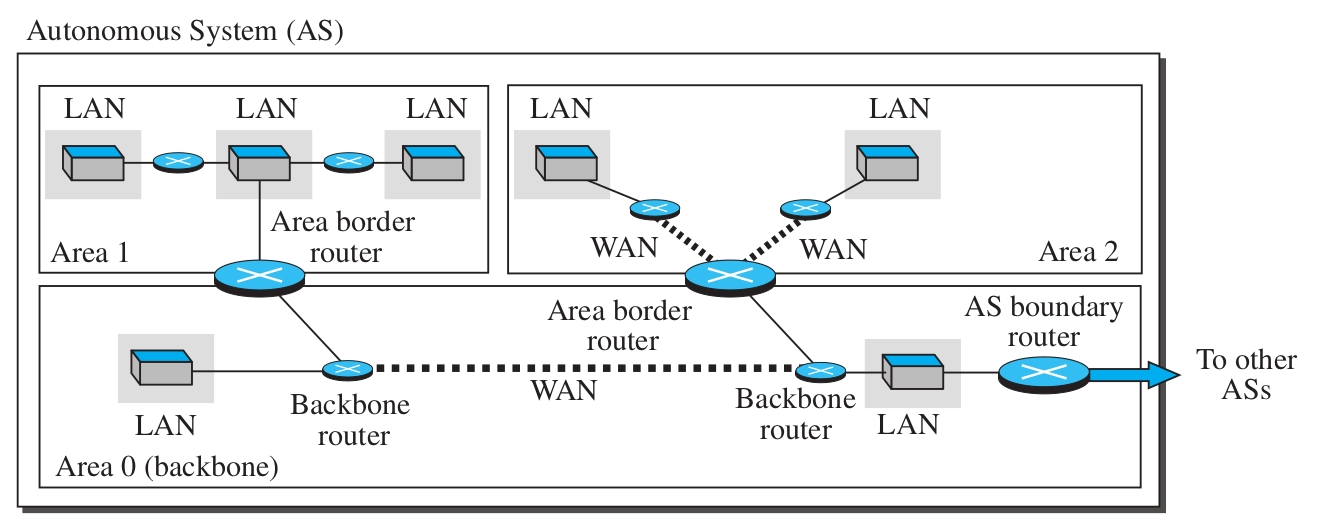
\includegraphics[width=0.9\linewidth]{figures/ospf}
	\caption{Autonomous System Hierarchy}
	\label{net2}
\end{figure}

\section{section1}
\lipsum[2] % Please comment this line and type in the introduction chapter


\subsection{title 2}
\lipsum[3] % Please comment this line and type in the introduction chapter

\noindent The system is described by the equation \ref{sys_eq1} below. Here y is the ordinate and x is the abscissa , m is the slope and c a constant.

\begin{equation} \label{sys_eq1}
y = mx + c
\end{equation}
\noindent Page centered and unnumbered multiple equations. The * symbol supresses equation numbering.
% Page centered and unnumbered equations
\begin{align*}
2x - 5y &=  8 \\ 
3x + 9y &=  -12
\end{align*}

\noindent Side by side figures can be created using this environment. See fig \ref{wave} below.
\begin{figure}[h!]
	\centering
	\begin{subfigure}[b]{0.4\textwidth}
		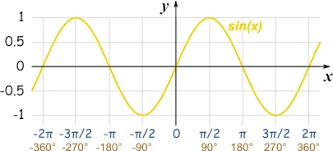
\includegraphics[width=\textwidth]{figures/sinewave}
		\caption{Sine Wave}
		\label{fig:1}
	\end{subfigure}
	\hspace{20mm}
	\begin{subfigure}[b]{0.4\textwidth}
		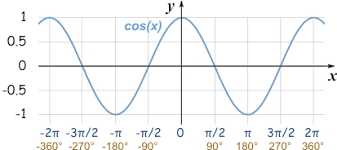
\includegraphics[width=\linewidth]{figures/cosine}
		\caption{Cosine Wave}
		\label{fig:2}
	\end{subfigure}
\caption{The Sine and Cosine waves}
\label{wave}
\end{figure}

%%********************Chapter 3**********
\chapter{Results}
\lipsum[10-15] % Please comment this line and type in the results chapter
	
\begin{table}[h!]
	\centering
	\caption{test table}
	\vspace*{5pt}
	\begin{tabular}{|c|c|c|}
		\hline
		Sl. No & Item 1 & Itm 2 \\ \hline
		1      & 37     & 45    \\ \hline
		2      & 42     & 23    \\ \hline
		3      & 47     & 1     \\ \hline
		4      & 52     & -21   \\ \hline
		5      & 57     & -43   \\ \hline
		6      & 62     & -65   \\ \hline
		7      & 67     & -87   \\ \hline
		8      & 72     & -109  \\ \hline
		9      & 77     & -131  \\ \hline
		10     & 82     & -153  \\ \hline
	\end{tabular}
\end{table}

%%********************Chapter 4**********
\chapter{Conclusion}
\lipsum[16-17] 

%%********************References**********
%%****This template uses IEEE bibliography style

 \begin{thebibliography}{99}
	\bibitem{AAC1} Abrar Ahmed Chhipa, et al., \emph{Adaptive Neuro-fuzzy Inference System Based Maximum Power Tracking Controller for Variable Speed WECS}, 2021 \textit{Energies}, Vol. 14, No. 19, pp.6275. https://doi.org/10.3390/en14196275
	
	\bibitem{AAC2} Abrar Ahmed Chhipa, et al., \emph{MPPT optimisation techniques and power electronics for renewable energy systems: wind and solar energy systems}, 2022 \textit{Int. J. Swarm Intelligence (IJSI)}, Vol. 7, No. 2. https://doi.org/10.1504/IJSI.2021.10041290
	
	\bibitem{AAC3} Abrar Ahmed Chhipa and Vinod Kumar, \emph{DC-Microgrid Voltage Regulation using Dual Active Bridge based SVR},\textit{2021 IEEE 7th International Conference on Electrical Energy Systems (ICEES)}, 2021, pp. 490-495, doi: 10.1109/ICEES51510.2021.9383696.
	
	\bibitem{AAC4} Abrar Ahmed Chhipa and Vinod Kumar, \emph{Grid-Connected PV System Power Forecasting Using Nonlinear Autoregressive Exogenous Model}, \textit{The 2nd Electric Power and Renewable Energy Conference (EPREC-2021)}, 28-30 May, 2021. (In Process)
	
	\bibitem{rpi}
	@online{ Raspberry pi,
		\url{https://www.raspberrypi.org/}
		Online; accessed 10-June-2019
	}
	
	\bibitem{japan} HU, Yun Chao, et al., \emph{Mobile edge computing?A key technology
		towards 5G}, ETSI white paper, 2015, vol. 11, no 11, p. 1-16.		
\end{thebibliography}

\end{document}